\documentclass[PICOReport.tex]{subfiles}

\begin{document}

The current cosmological model, as encoded by $\Lambda$CDM, provides a good fit to most current data. A host of cosmological observations including the CMB fit within the model that consists of only six parameters~\citep{Planck2018_I}. But the model is phenomenological and it leaves fundamental questions open. Premier among them is the unknown content of the majority of the Universe. Approximately 95\% of the Universe appears to be composed of dark matter and dark energy of unknown nature, both of which are necessary to explain observations at scales ranging from that of a galaxy to that of the Hubble volume. Yet, there are no detection of dark matter particles, and as for dark energy, it even lacks a compelling theoretical motivation.

In this context, tension between measurements of any $\Lambda$CDM parameter obtained by different probes compel additional stringent tests and investigation of alternatives to the prevailing paradigm. Examples of emerging tensions are: the $3.6\sigma$ discrepancy between the CMB- and local-Universe-anchored supernovae-based measurements of the Hubble constant~\citep{Aghanim:2018eyx,Riess2018}; the identification of lack of correlations at large angles in the $TT$ power spectrum that has an apparent probability of less than $10^{-3}$ of occurrence in standard $\Lambda$CDM~\citep{TT_correlations}; and the $\sim 2\sigma$ tension in measurements of the amplitude of late time perturbations $\sigma_{8}$ between the \planck\ CMB $TT$, $TE$, and $EE$ power spectra and those from cosmic shear surveys~\citep{Joudaki+2017, Abbott+2018, Hikage+2018, vanUitert+2018}.  A similar level  of tension for $\sigma_{8}$ ($\sim2\sigma$) arises when comparing \planck\ CMB spectra and cluster counts from \planck\ and other surveys~\citep{Planck, Bocquet+2018}. Such tensions, while perhaps only indicating the presence of systematic effects in the measurements, may in fact point toward new physics. One way to search for new physics is to better constrain the current measurements and the known extensions beyond the base six-parameter set. 

Given an experiment's baseline noise and angular resolution, and an input set of $N$ parameters, it is straightforward to calculate the uncertainty with which it will constrain the set~\citep{core_parameter}. A figure of merit (FOM) that quantifies the strength of the constraint is the volume of the uncertainty region in the $N$-dimensional parameter space. We use the same analytical approach and FOM that have also been used in other studies~\citep{core_parameter,Wang2008,pdg2018,Namikawa2010}.\footnote{The FOM is determined by the covariance of the Fisher information matrix, ${\rm FOM} = \left( \det \left[ \mbox{cov} ( p_i)  \right] \right)^{-1/2},\,\, i=1, ..., N$, where $p$ is the parameter set.} This FOM is defined such that a larger value linearly corresponds to {\it smaller} volume and thus to smaller parameter errors. 

Fig.~\ref{fig:fom} shows the increase in the FOM since \cobe\ for the six-parameter $\Lambda$CDM model, as well as for additional cosmological parameters.\footnote{The six-parameter $\Lambda$CDM model includes: the baryon density; the dark matter density; the amplitude and spectral index of a power-law spectrum of initial perturbations; the angular scale of acoustic oscillations; and the optical depth to reionization.} The Figure only includes data from CMB experiments. The FOM for $\Lambda$CDM improved by a factor of 100 between {\it WMAP} and \planck , and will further improve by a factor of $10^{5}$ with PICO. For the 11-parameter set that includes $\Neff$ shown in the Figure PICO will improve upon \planck\ by a factor of $0.5\times10^{9}$. Having achieved this improvement, there would be only little information left to extract with this parameter set even by a mission with double the resolution and nearly ten times lower noise (Fig.~\ref{fig:fom}). Even stronger FOM improvements are obtained when a 12-parameter set is considered~\citep{picoweb_lcdm}, and when the PICO CMB data will be combined with data sets available in the next decade, including weak lensing, BAO, and cluster of galaxies. 

 \begin{figure}%[t,h]
\hspace{-0.2in}
\parbox{2.7in}{\centerline {
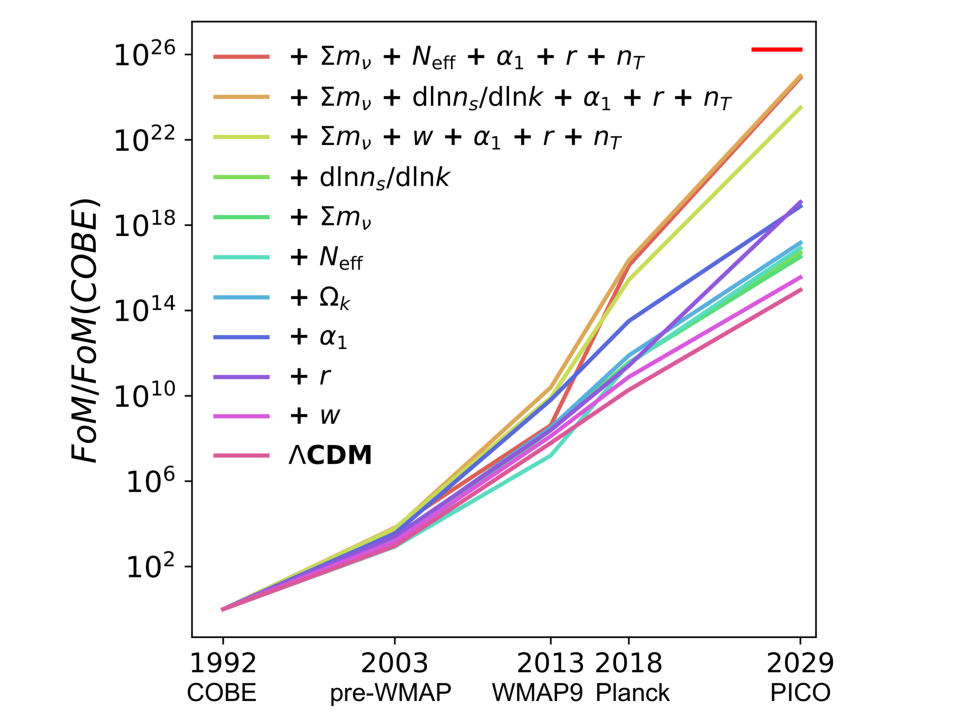
\includegraphics[width=3.0in]{images/fom_plot_CVL+del.pdf} } }
%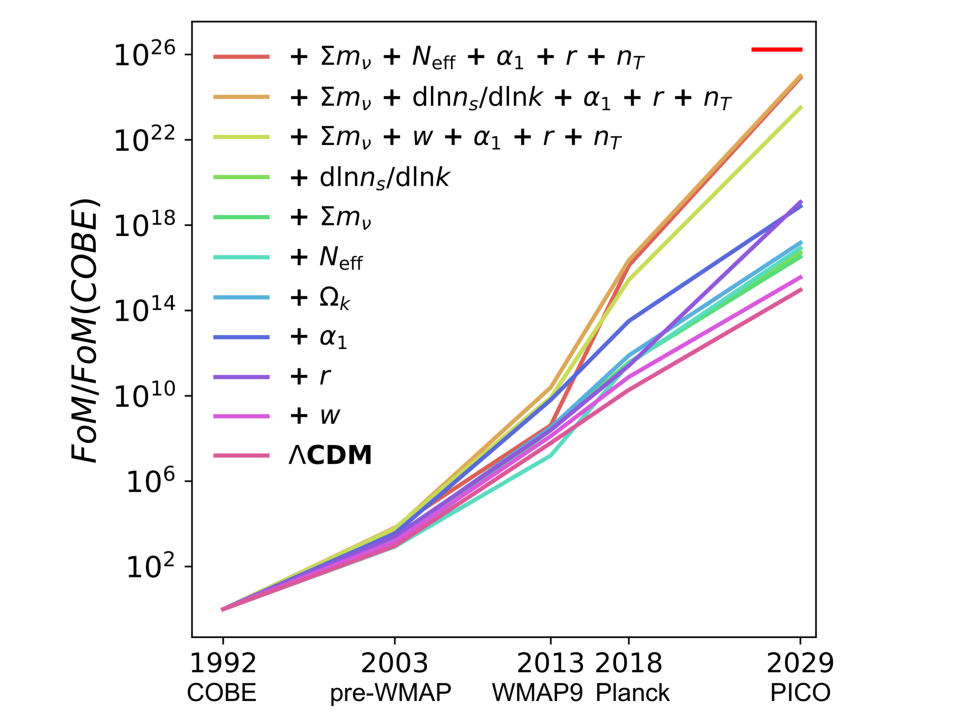
\includegraphics[width=3.0in]{images/fom_plot_CVL+del.pdf} } }
\hspace{0.in}
\parbox{3.8in}{
\caption{\captiontext 
The increase in the FOM using data from CMB experiments since \cobe\ for the $\Lambda$CDM six-parameter model (dark purple) and when adding other cosmological parameters.  Increase in value represents increase in information content. PICO data will continue the average trend (blue line, $\Lambda$CDM + $\alpha_{1}$) of doubling the FOM every 10 months since 1992. For an 11-parameter set that includes $\Neff$ (red increasing line) PICO will improve the FOM by a factor of $0.5\times10^{9}$ relative to \planck , and will extract nearly the same information as that attainable by a mission with double the resolution and nine times lower baseline noise (top right red horizontal bar). The 11-parameter set includes: $w$-dark energy; $r$-the tensor to scalar ratio; $\alpha_{1}$-amplitude of correlated CDM isocurvature perturbations; $\Omega_{k}$-curvature; $\Neff$-effective number of light relics; $\sum m_{\nu}$-sum of neutrino masses; and $d\ln n_{s}/d\ln k$-running of the spectral index.   
\label{fig:fom} } }
\vspace{-0.13in}
\end{figure}

These improvements will test $\Lambda$CDM so stringently that it is hard to imagine it surviving such a scrutiny if it is not fundamentally correct. If tensions deepen to become discrepancies, it would be even more exciting if a new cosmological model emerged. 


\end{document}

%The improvement of the FoM \emph{with CMB alone}, by a factor between $3$ and $10$ billions (when $r$ is included in the extra parameters) or close to five million (excluding $r$) provides a test of $\Lambda$CDM that, is so stringent that it is hard to imagine that $\Lambda$CDM can survive such a scrutiny if it is not fundamentally correct. This is true in particular considering that in parallel to the improvement of CMB constraints, other probes such as weak lensing, BAO, clusters of galaxies (the later with PICO itself), will also experiment similar tightening of their own error boxes based on largely independent observables.

%PICO, in addition, will also improve constraints on other extensions of $\Lambda$CDM, such as interacting dark matter (with constraints on scattering cross sections), modifications of the laws of gravitation, primordial non-Gaussianity, etc. The history of the development of physical cosmology has taught us that discoveries often come from unexpected directions. PICO is ideally suited to look at the surprises that the Universe still has to reveal.

%\begin{table*}
%\begin{center}\footnotesize
%\begin{tabular}{cccc}
%\hline \hline
%    Model     & PICO v4.0 & PICO v4.1 &  Planck18   \\                   
%\hline
%$\Lambda$CDM + $\neff$ +$\alpha_1$+$w_0$+$w_a$+$\mnu$ & $7.4\times10^{6}$ & $4.8\times10^{6}$& $1$  \\
%$\Lambda$CDM + $\neff$ +$\alpha_1$+$w_0$+$w_a$+$r$+$\mnu$ & $2.7\times10^{10}$ & $9.5\times10^{9}$& $1$  \\
%\hline
%\hline
%\end{tabular}
%%\caption{}
%\label{tabFoM}
%\end{center}
%\end{table*}



%%%%%%%%%%%%%%%%%%%%%%%%%%%%%%%
